\documentclass[10pt]{article}

\usepackage[left=0.85in, right=0.85in, top=0.9in, bottom=0.9in]{geometry}

\usepackage{subcaption}

% Import MathDesign (this brings along Bitstream Charter)
\usepackage[bitstream-charter]{mathdesign}
\usepackage{amsmath}
\usepackage[scaled=0.92]{PTSans}

\usepackage{titling}

% COLOR
\usepackage[table,dvipsnames]{xcolor}
\definecolor{shadecolor}{gray}{0.9}

% SPACING and TEXT
\usepackage[final,expansion=alltext]{microtype}
\pdfoutput=1

\usepackage[parfill]{parskip}
\usepackage{setspace}
\setlength{\parskip}{3pt plus 1pt minus 1pt}

% FIGURES
\usepackage{graphicx}
\usepackage[labelfont={it, small}, font=small, skip=4pt]{caption}

% HYPERREF
\usepackage[colorlinks,linktoc=all]{hyperref}
\hypersetup{citecolor=MidnightBlue}
\hypersetup{linkcolor=black}
\hypersetup{urlcolor=MidnightBlue}

% CLEVEREF must come after HYPERREF
\usepackage[nameinlink]{cleveref}

% MATH
\usepackage{booktabs}
\DeclareRobustCommand{\mb}[1]{\boldsymbol{#1}}

% Compact sections
\usepackage{titlesec}
\titlespacing*{\section}{0pt}{8pt}{4pt}
\titlespacing*{\subsection}{0pt}{6pt}{2pt}

% -----------------------------------------------------------------------
\title{\textbf{Coding Assignment 3: SLAM and Motion Planning}}
\author{CS\,188: Introduction to Robotics \quad--\quad Winter 2026}
\date{}

\begin{document}
\maketitle
\vspace{-1.5em}
\thispagestyle{empty}

% ===================================================================
\section{Part A: EKF-SLAM Trajectory and Uncertainty}
% ===================================================================

\subsection{A1.\ Path Design: Which Trajectory is Better for SLAM?}

I tested two different control strategies in the same 15-landmark environment:
\begin{itemize}\itemsep=0pt
  \item \textbf{Path~A (Greedy Forward):} L-shaped sweep. Straight east for 150~steps, turn left, straight north for 150~steps, turn left, then west. Each landmark is observed once or twice.
  \item \textbf{Path~B (Looping Revisit):} Heads northeast, then enters tight circular orbits ($\omega{=}0.25$~rad/s), translates, and does a second orbit. Landmarks near the orbit centres are observed 4--8 times.
\end{itemize}

\begin{figure}[ht]
\centering
\begin{subfigure}[t]{0.46\textwidth}
  \centering
  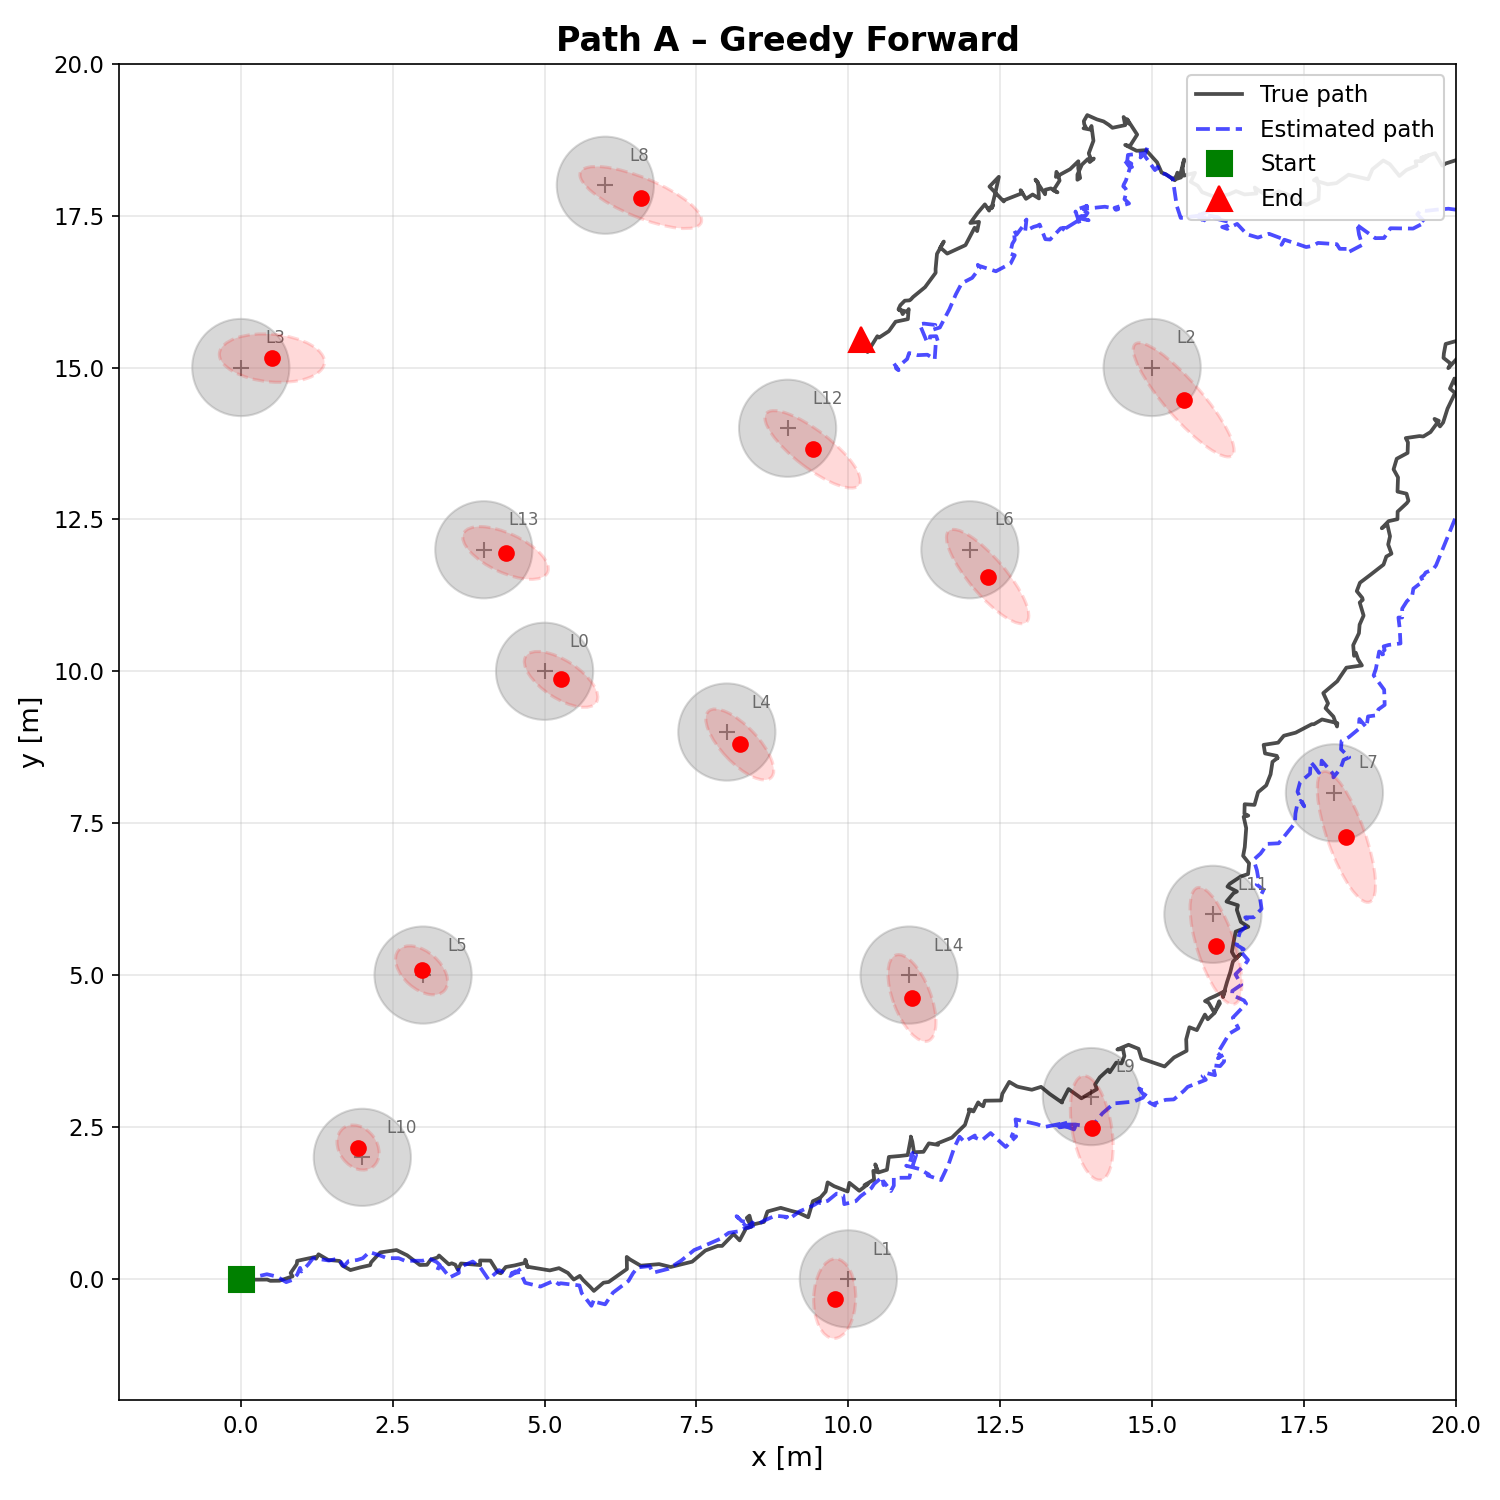
\includegraphics[width=\textwidth]{results/partA/a1_path_a.png}
  \caption{Path~A: Greedy Forward.}
\end{subfigure}
\hfill
\begin{subfigure}[t]{0.46\textwidth}
  \centering
  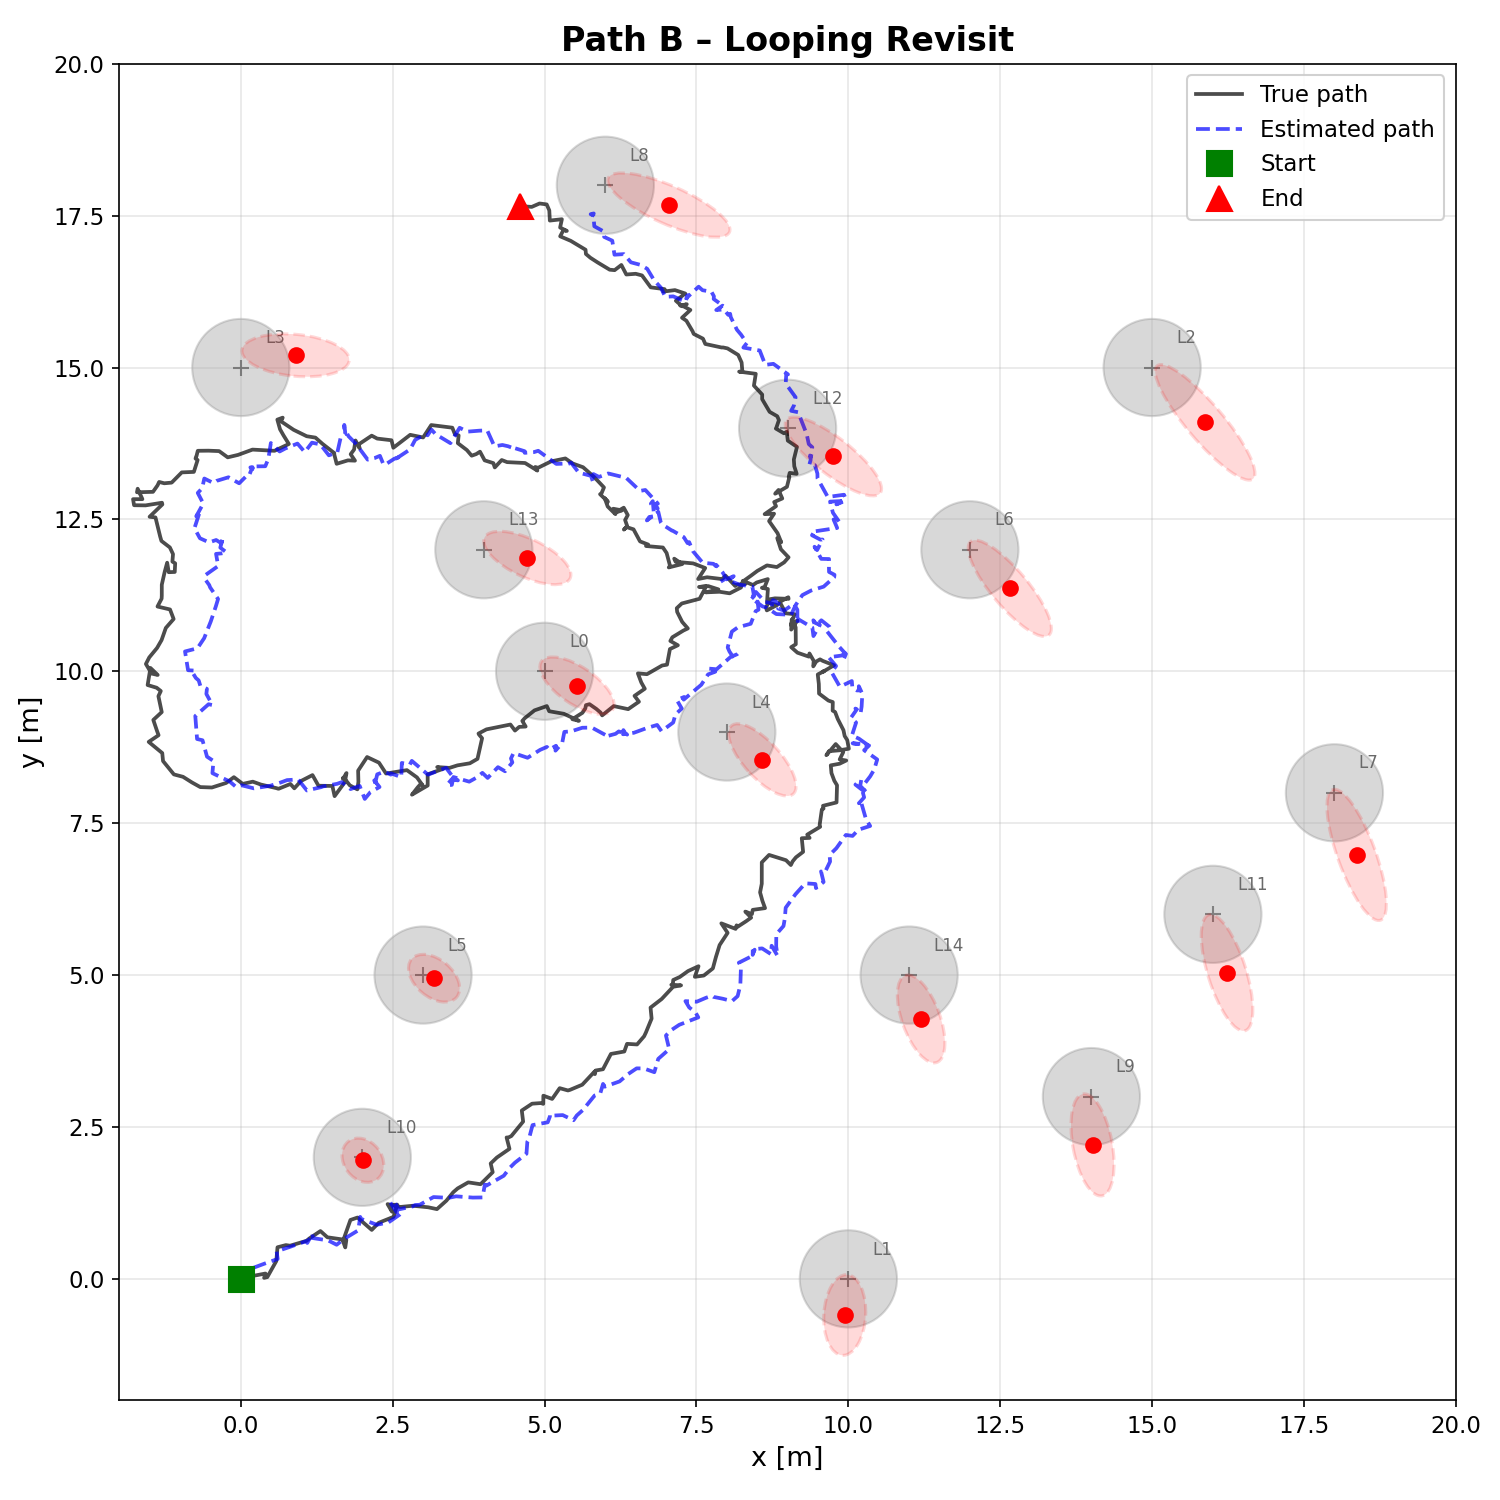
\includegraphics[width=\textwidth]{results/partA/a1_path_b.png}
  \caption{Path~B: Looping Revisit.}
\end{subfigure}
\caption{True path (black) vs.\ estimated path (blue dashed) with landmark $2\sigma$ ellipses. Green square = start, red triangle = end.}
\label{fig:a1-traj}
\end{figure}

\begin{table}[ht]
\centering\small
\begin{tabular}{@{}lcc@{}}
\toprule
\textbf{Metric} & \textbf{Greedy Forward} & \textbf{Looping Revisit} \\
\midrule
Final pose error & 0.669\,m & 1.204\,m \\
Mean pose error & 0.837\,m & 0.775\,m \\
Final pose uncertainty & 0.572\,m & 0.607\,m \\
Final avg landmark unc. & 0.215 & 0.217 \\
Landmarks observed & 15/15 & 15/15 \\
\bottomrule
\end{tabular}
\caption{A1 trajectory comparison (500 steps, medium noise).}
\label{tab:a1}
\end{table}

Greedy Forward has a lower \emph{final} pose error (0.669 vs.\ 1.204\,m), but Looping has a lower \emph{mean} error (0.775 vs.\ 0.837\,m). This is because the looping path keeps re-observing landmarks, which triggers EKF corrections that pull the estimate back toward truth. The greedy path drifts during long straight segments but happens to end near landmarks that anchor the final estimate. Both paths observe all 15 landmarks, so final landmark uncertainties are nearly identical ($\approx 0.215$).

\paragraph{Uncertainty ellipse evolution.}
\cref{fig:snapshots} shows map snapshots at steps 50, 150, 250, 350, and 500. Each dot is an observed landmark. The colour encodes uncertainty: blue means confident, red means uncertain. The ellipse around each dot is the $2\sigma$ confidence region. A large ellipse means the EKF is unsure where the landmark is.

Under Path~A, ellipses shrink when a landmark is first observed but stay the same size after that, because the robot moves on and never returns. Under Path~B, landmarks near the orbit centre are re-observed on every loop. Each re-observation triggers an EKF update where the Kalman gain uses the cross-covariance to correct both the robot pose and landmark position. The ellipses visibly collapse from large red shapes (step~50) to tight blue dots (step~350). This is the \textbf{loop-closure effect}, the most important mechanism in EKF-SLAM for reducing uncertainty.

\begin{figure}[ht]
\centering
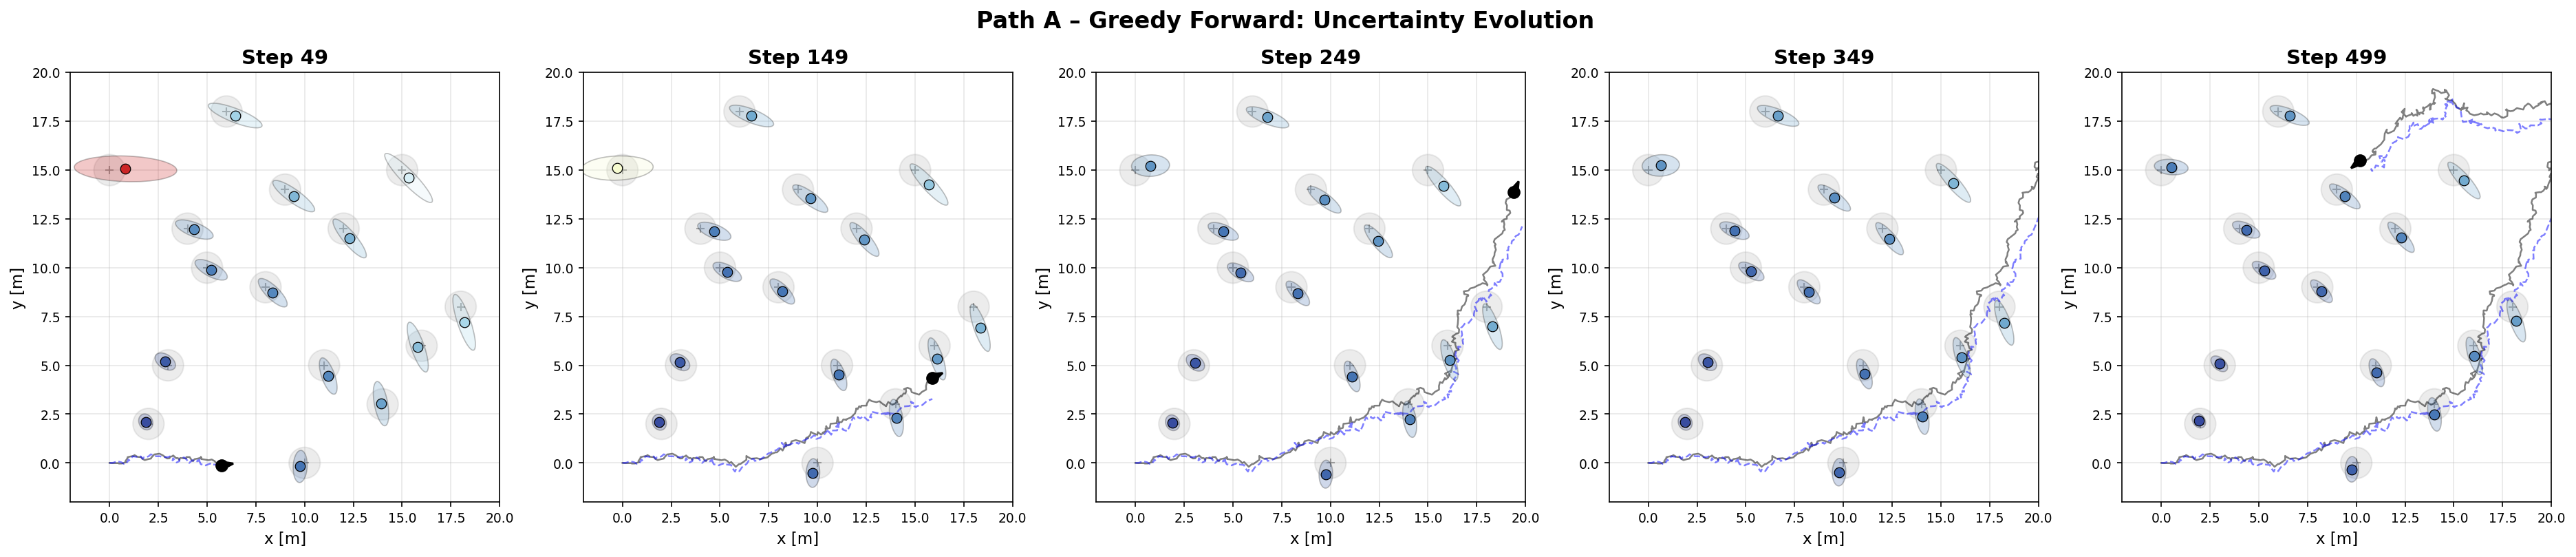
\includegraphics[width=\textwidth]{results/partA/a1_snapshots_path_a.png}\\[2pt]
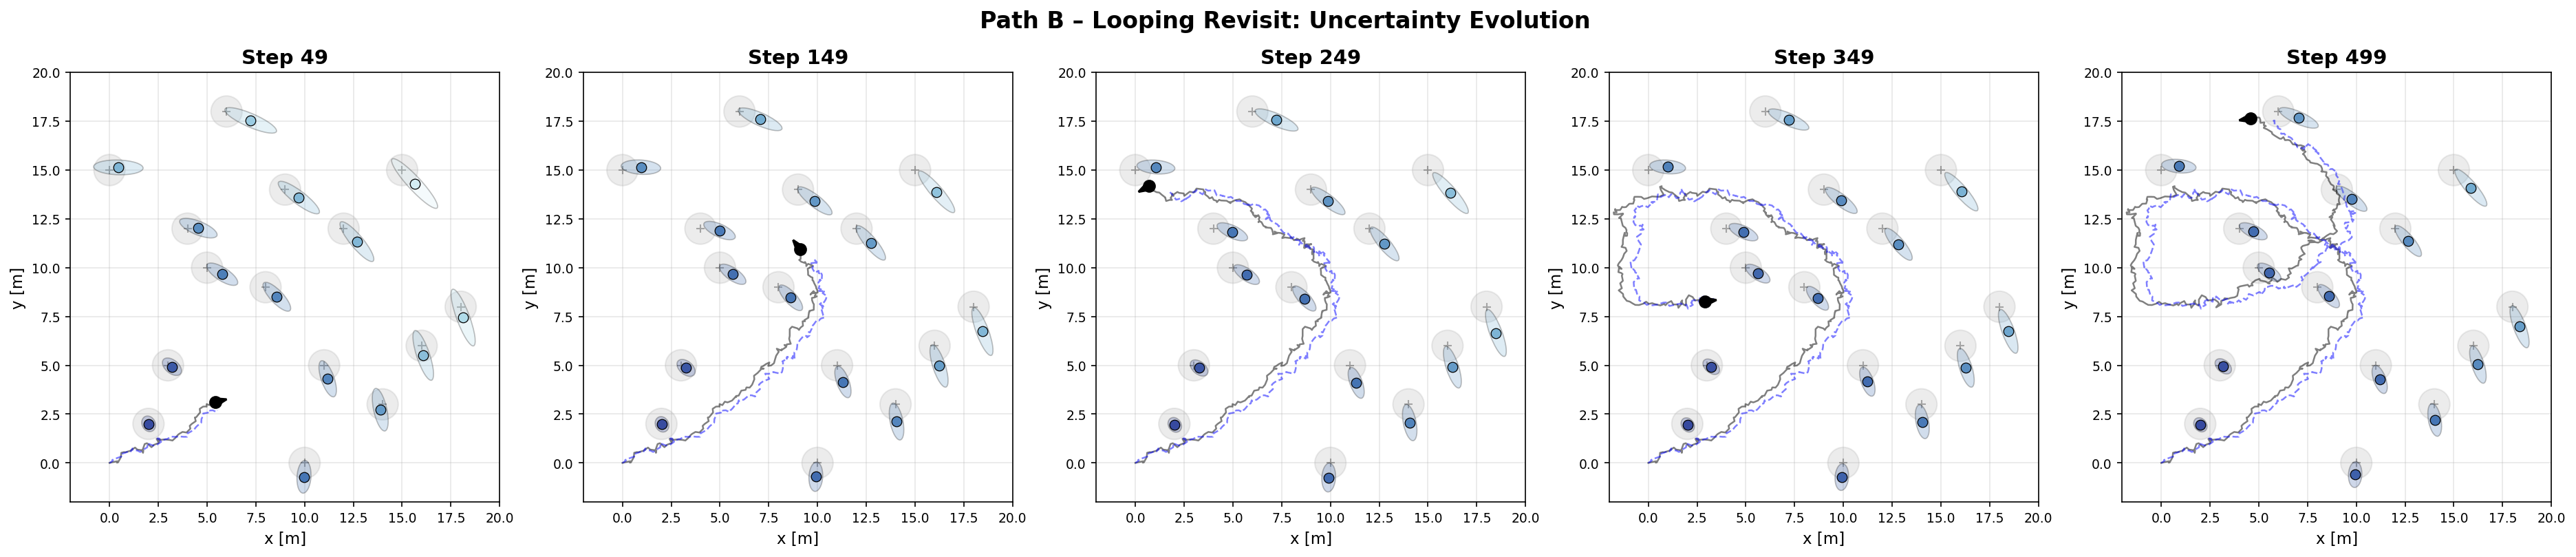
\includegraphics[width=\textwidth]{results/partA/a1_snapshots_path_b.png}
\caption{Uncertainty snapshots. \textit{Top:} Path~A, ellipses stay fixed after first observation. \textit{Bottom:} Path~B, ellipses collapse with repeated re-observation. Landmarks far from the orbit (e.g.\ top-right) keep larger ellipses.}
\label{fig:snapshots}
\end{figure}

% -------------------------------------------------------------------
\subsection{A2.\ Noise Sensitivity}

I used Path~B for all noise experiments because it is the stronger baseline.

\begin{table}[ht]
\centering\small
\begin{tabular}{@{}lccc@{\qquad}lccc@{}}
\toprule
\textbf{R Level} & $\sigma_{xy}$ & $\sigma_\theta$ & \textbf{Pose Err}
& \textbf{Q Level} & $\sigma_r$ & $\sigma_b$ & \textbf{Pose Err} \\
\midrule
Low & 0.05 & $1.5^\circ$ & 0.278\,m & Low & 0.2 & $3.0^\circ$ & 1.263\,m \\
Med & 0.10 & $3.0^\circ$ & 1.204\,m & Med & 0.5 & $8.0^\circ$ & 1.204\,m \\
High & 0.30 & $8.0^\circ$ & 1.857\,m & High & 1.5 & $15.0^\circ$ & 1.351\,m \\
\bottomrule
\end{tabular}
\caption{Noise sensitivity. Left: varying process noise $\mb{R}$ (Q fixed). Right: varying measurement noise $\mb{Q}$ (R fixed).}
\label{tab:a2}
\end{table}

\textbf{Process noise is far more damaging.} Increasing R-std by $6\times$ causes $6.7\times$ more error, while increasing Q-std by $7.5\times$ causes only $1.1\times$ more error. Process noise corrupts the robot state at every predict step (500 total), so drift accumulates between observations. Measurement noise only degrades the quality of individual corrections and gets averaged out by repeated observations. Even under high measurement noise, the looping path stays at 1.351\,m error. This confirms that revisiting landmarks gives built-in protection against sensor noise.

\begin{figure}[ht]
\centering
\begin{subfigure}[t]{0.48\textwidth}
  \centering
  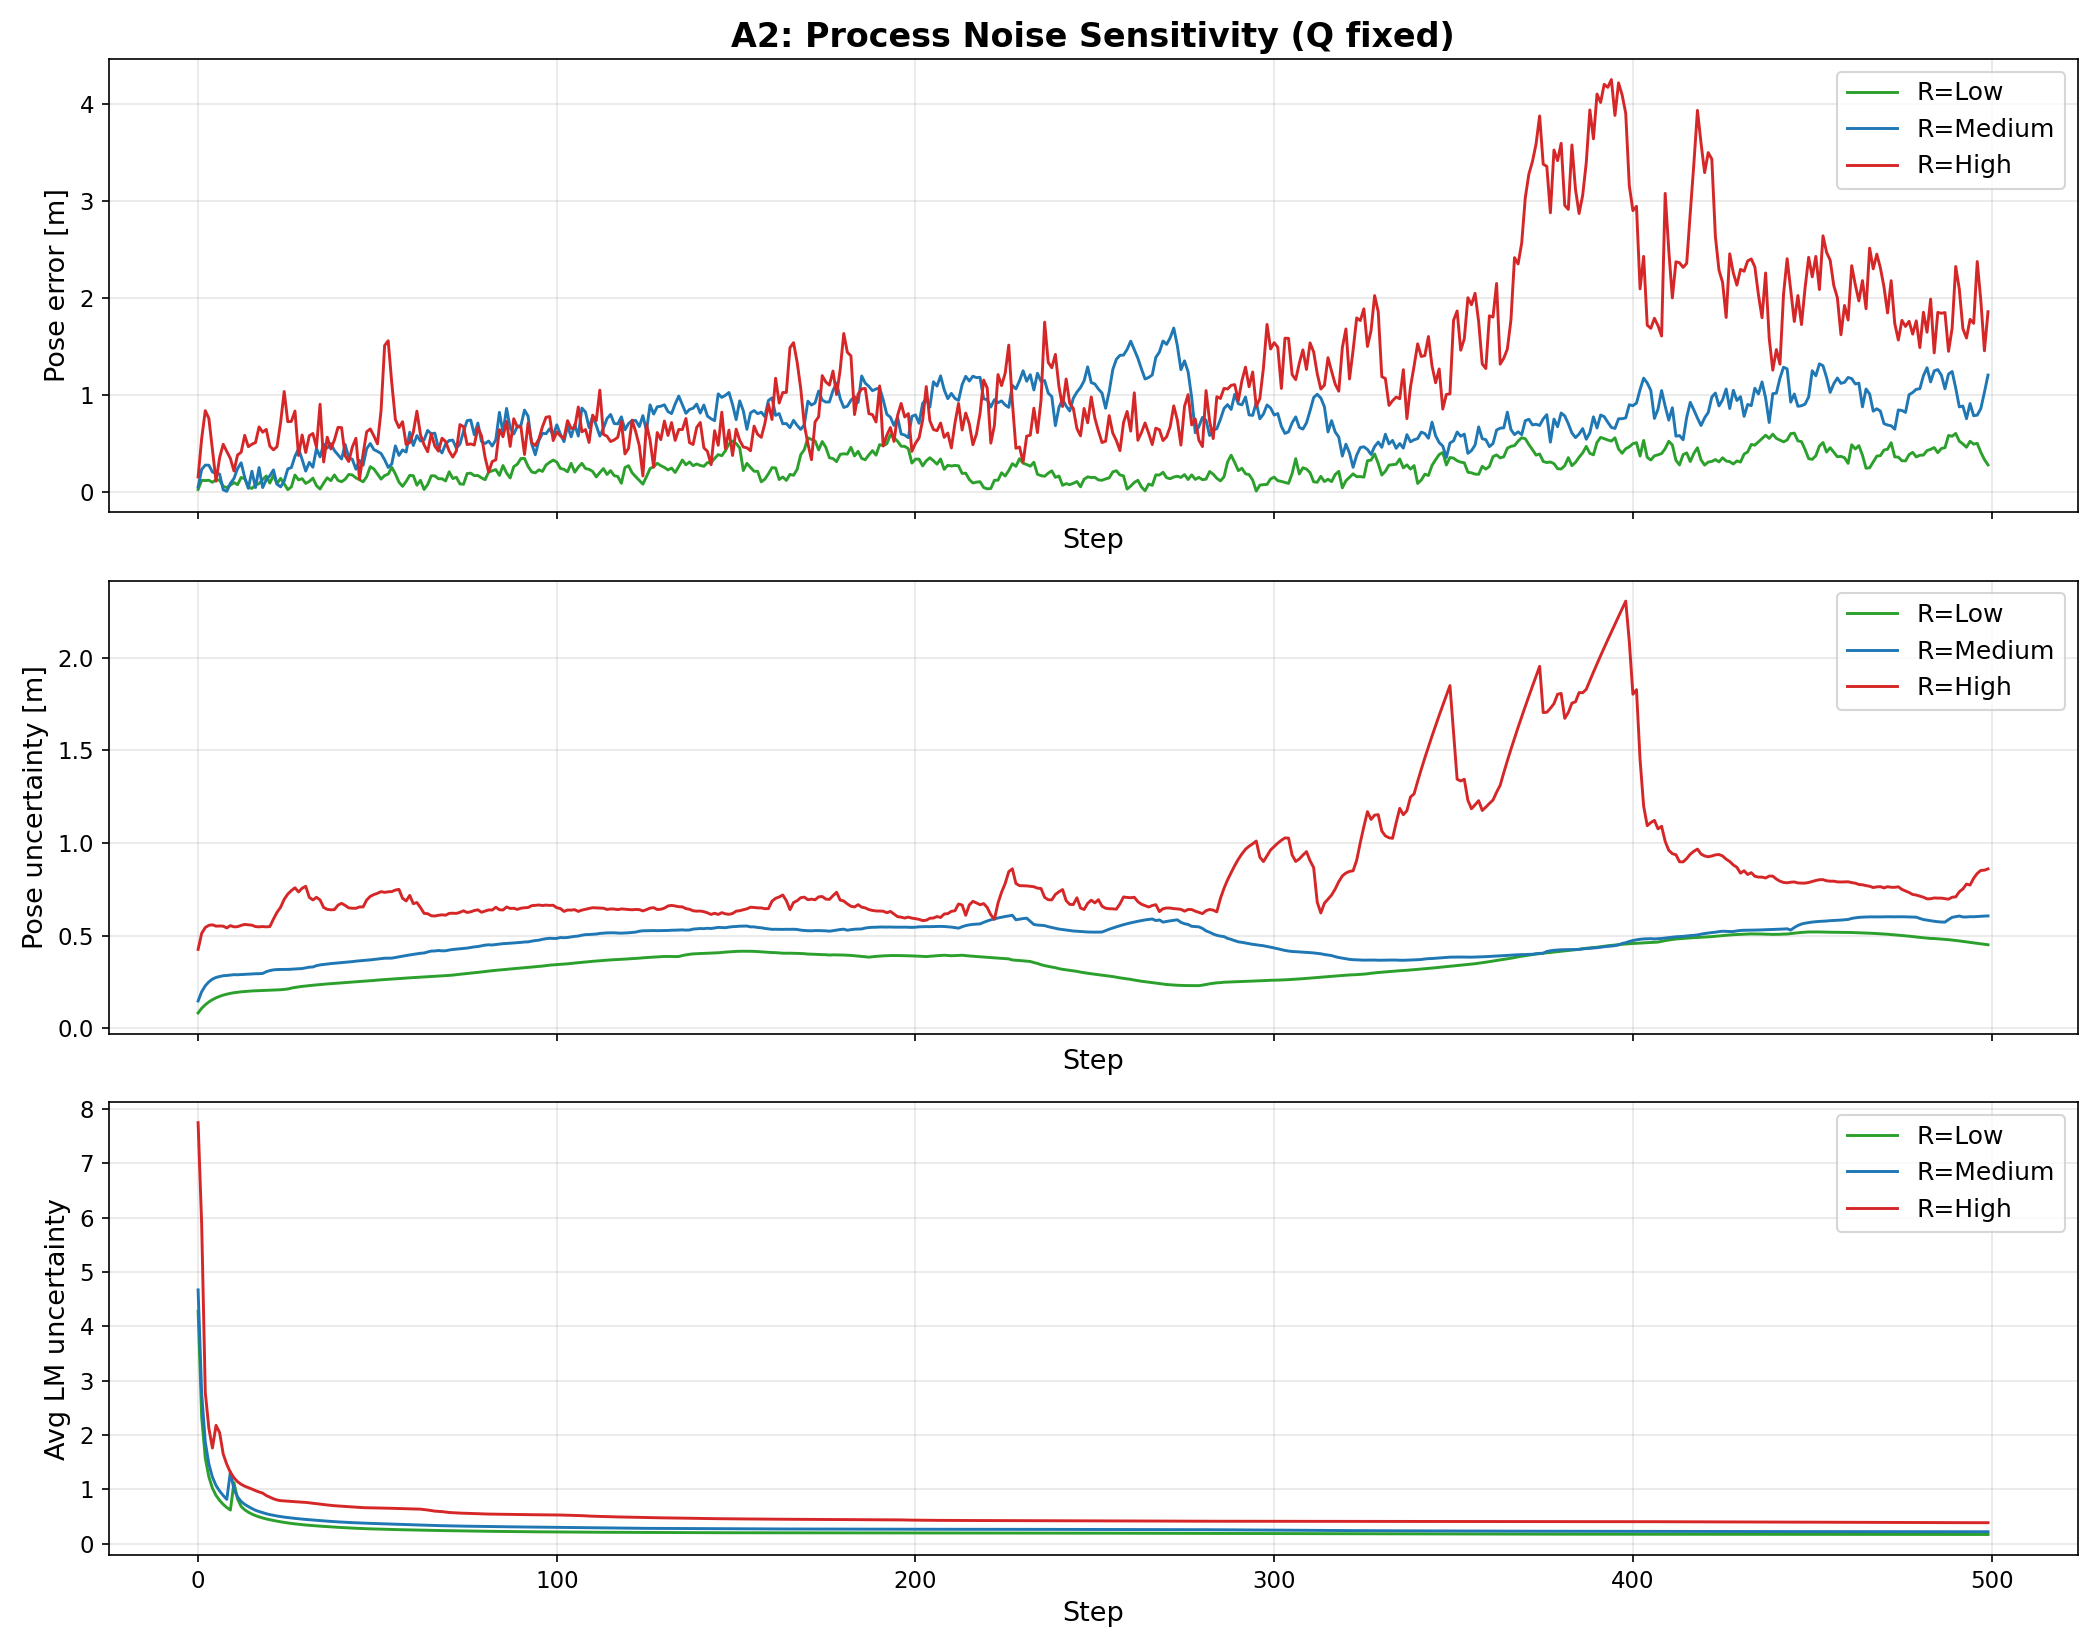
\includegraphics[width=\textwidth]{results/partA/a2_process_noise.png}
  \caption{Process noise sweep ($\mb{Q}$ fixed).}
\end{subfigure}
\hfill
\begin{subfigure}[t]{0.48\textwidth}
  \centering
  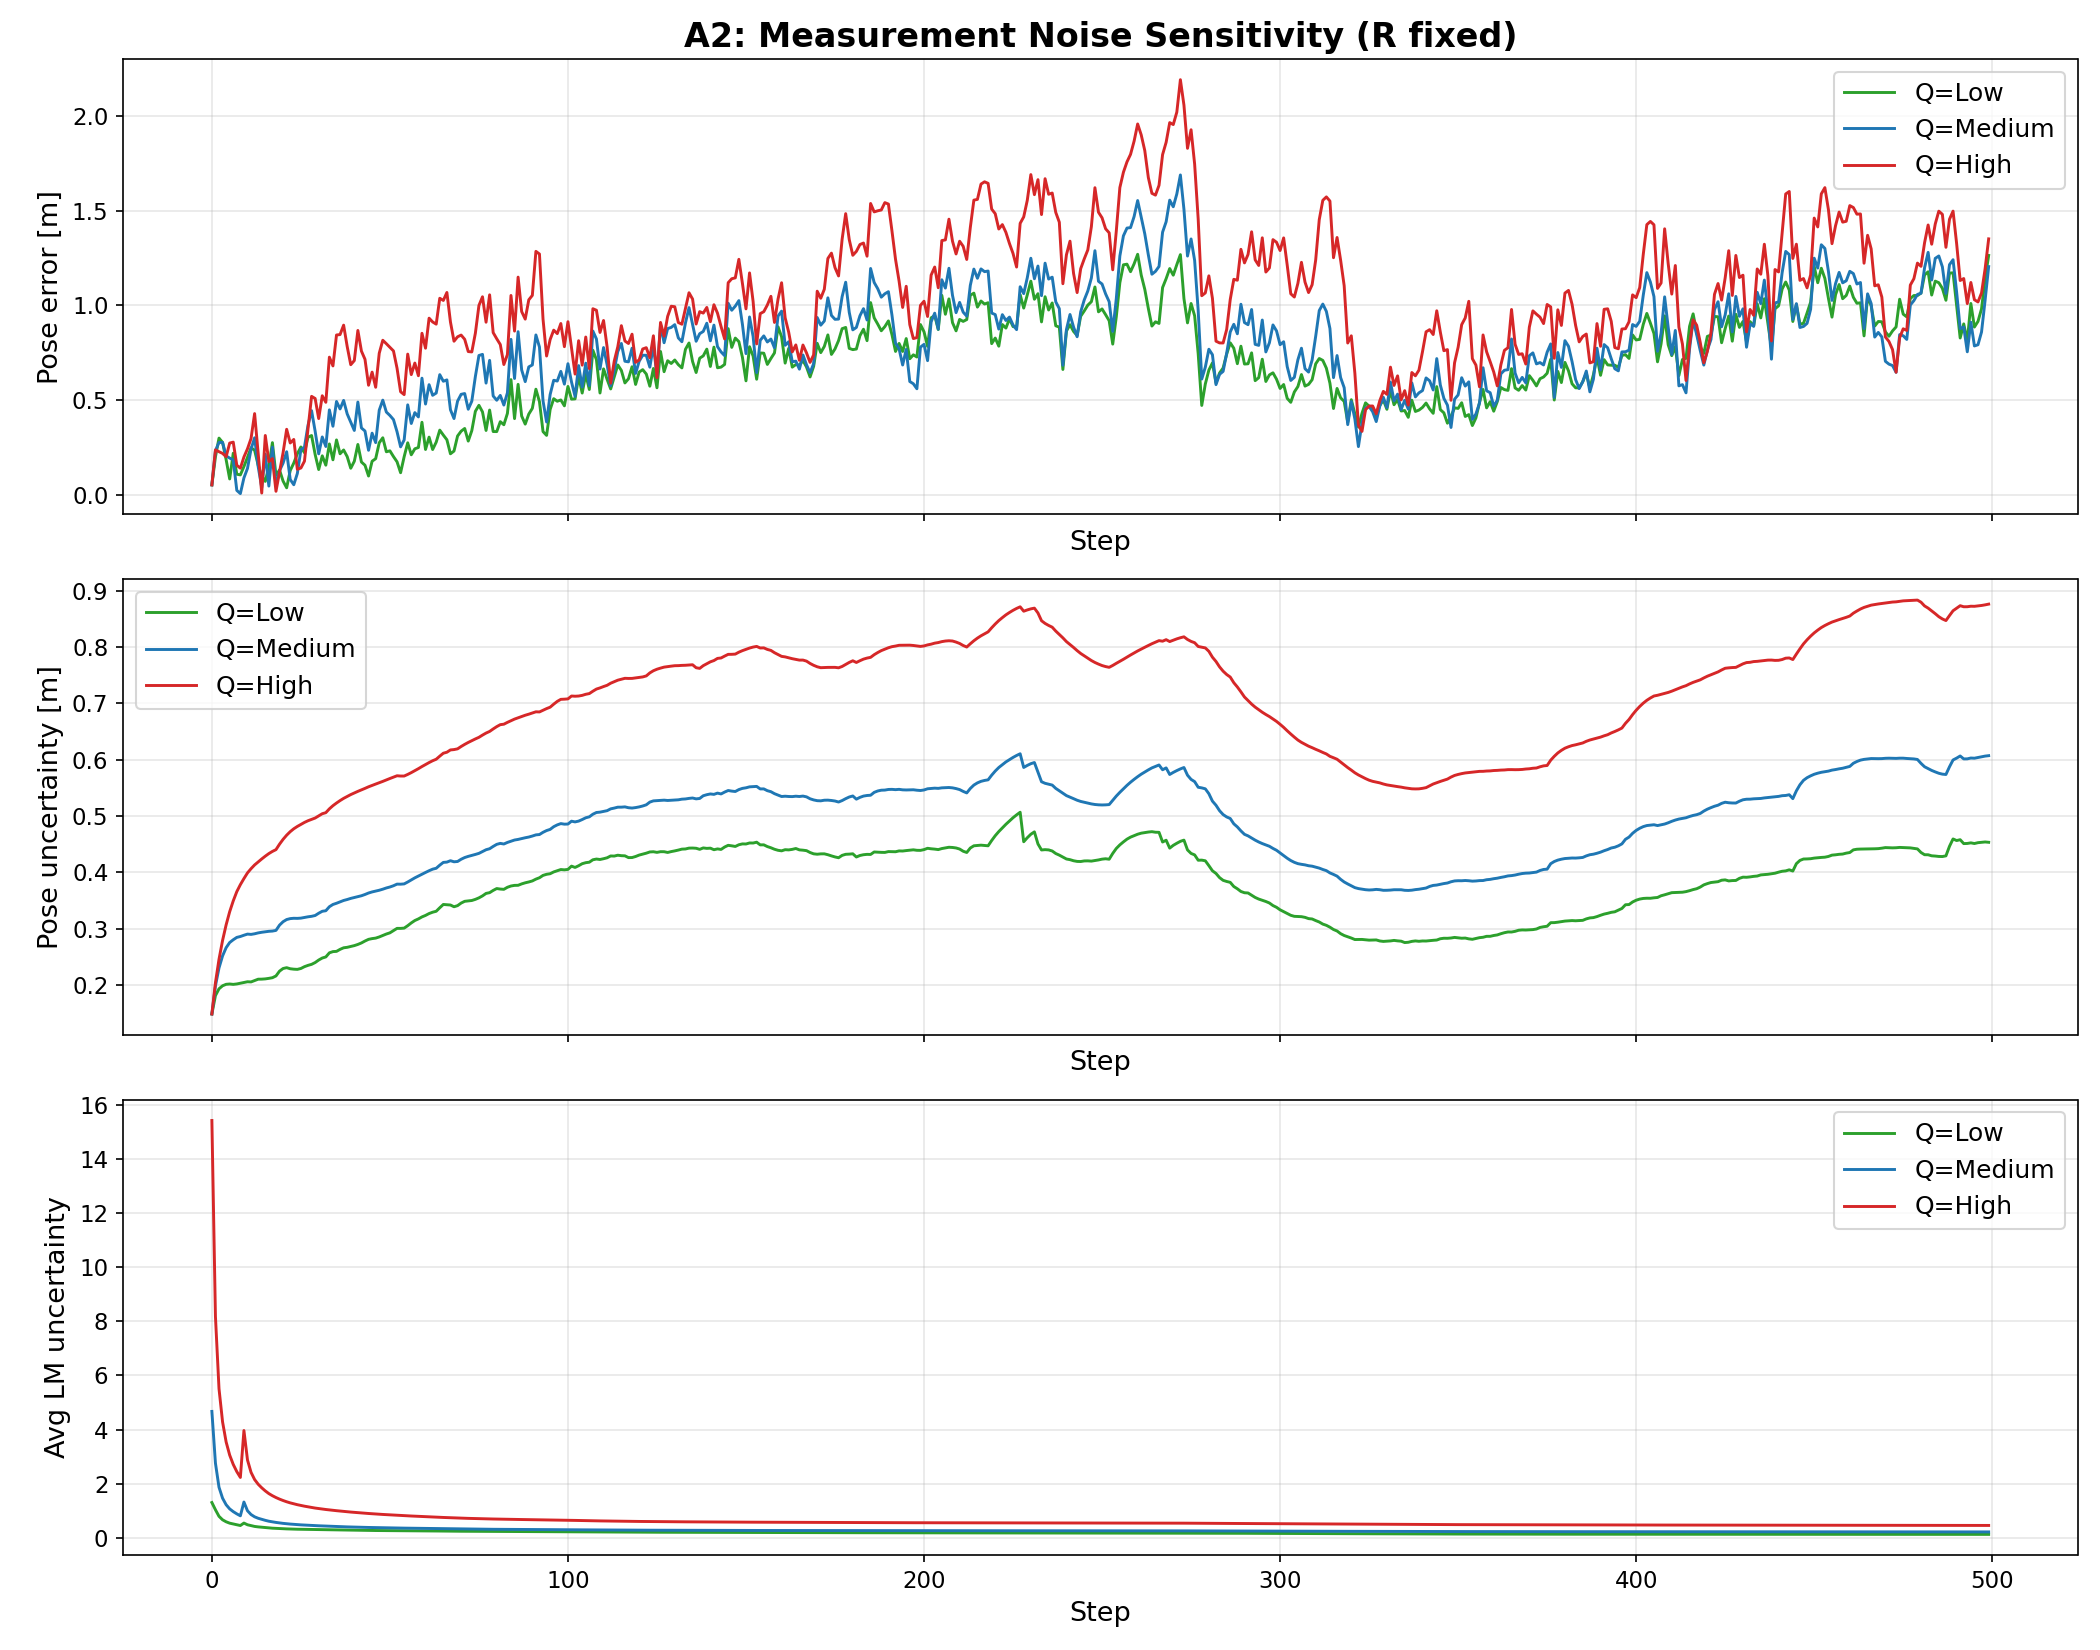
\includegraphics[width=\textwidth]{results/partA/a2_measurement_noise.png}
  \caption{Measurement noise sweep ($\mb{R}$ fixed).}
\end{subfigure}
\caption{A2 noise sensitivity. Higher process noise (left, red) is much worse across all metrics. Measurement noise (right) has a smaller effect.}
\label{fig:a2-noise}
\end{figure}

% ===================================================================
\section{Part B: PRM vs RRT Planning Comparison}
% ===================================================================

\subsection{B1.\ Start/Goal Scenarios}
\begin{itemize}\itemsep=0pt
  \item \textbf{Scenario~1 (Open):} Obstacle radius 0.8, start$=[1,1]$, goal$=[19,1]$. Wide gaps between obstacles.
  \item \textbf{Scenario~2 (Constrained):} Obstacle radius 1.0, start$=[1,1]$, goal$=[17,17]$. Tight passages.
\end{itemize}
\textbf{Prediction:} PRM should give shorter paths (A* on roadmap) but be slower. RRT may struggle with narrow passages but should be faster.

\begin{figure}[ht]
\centering
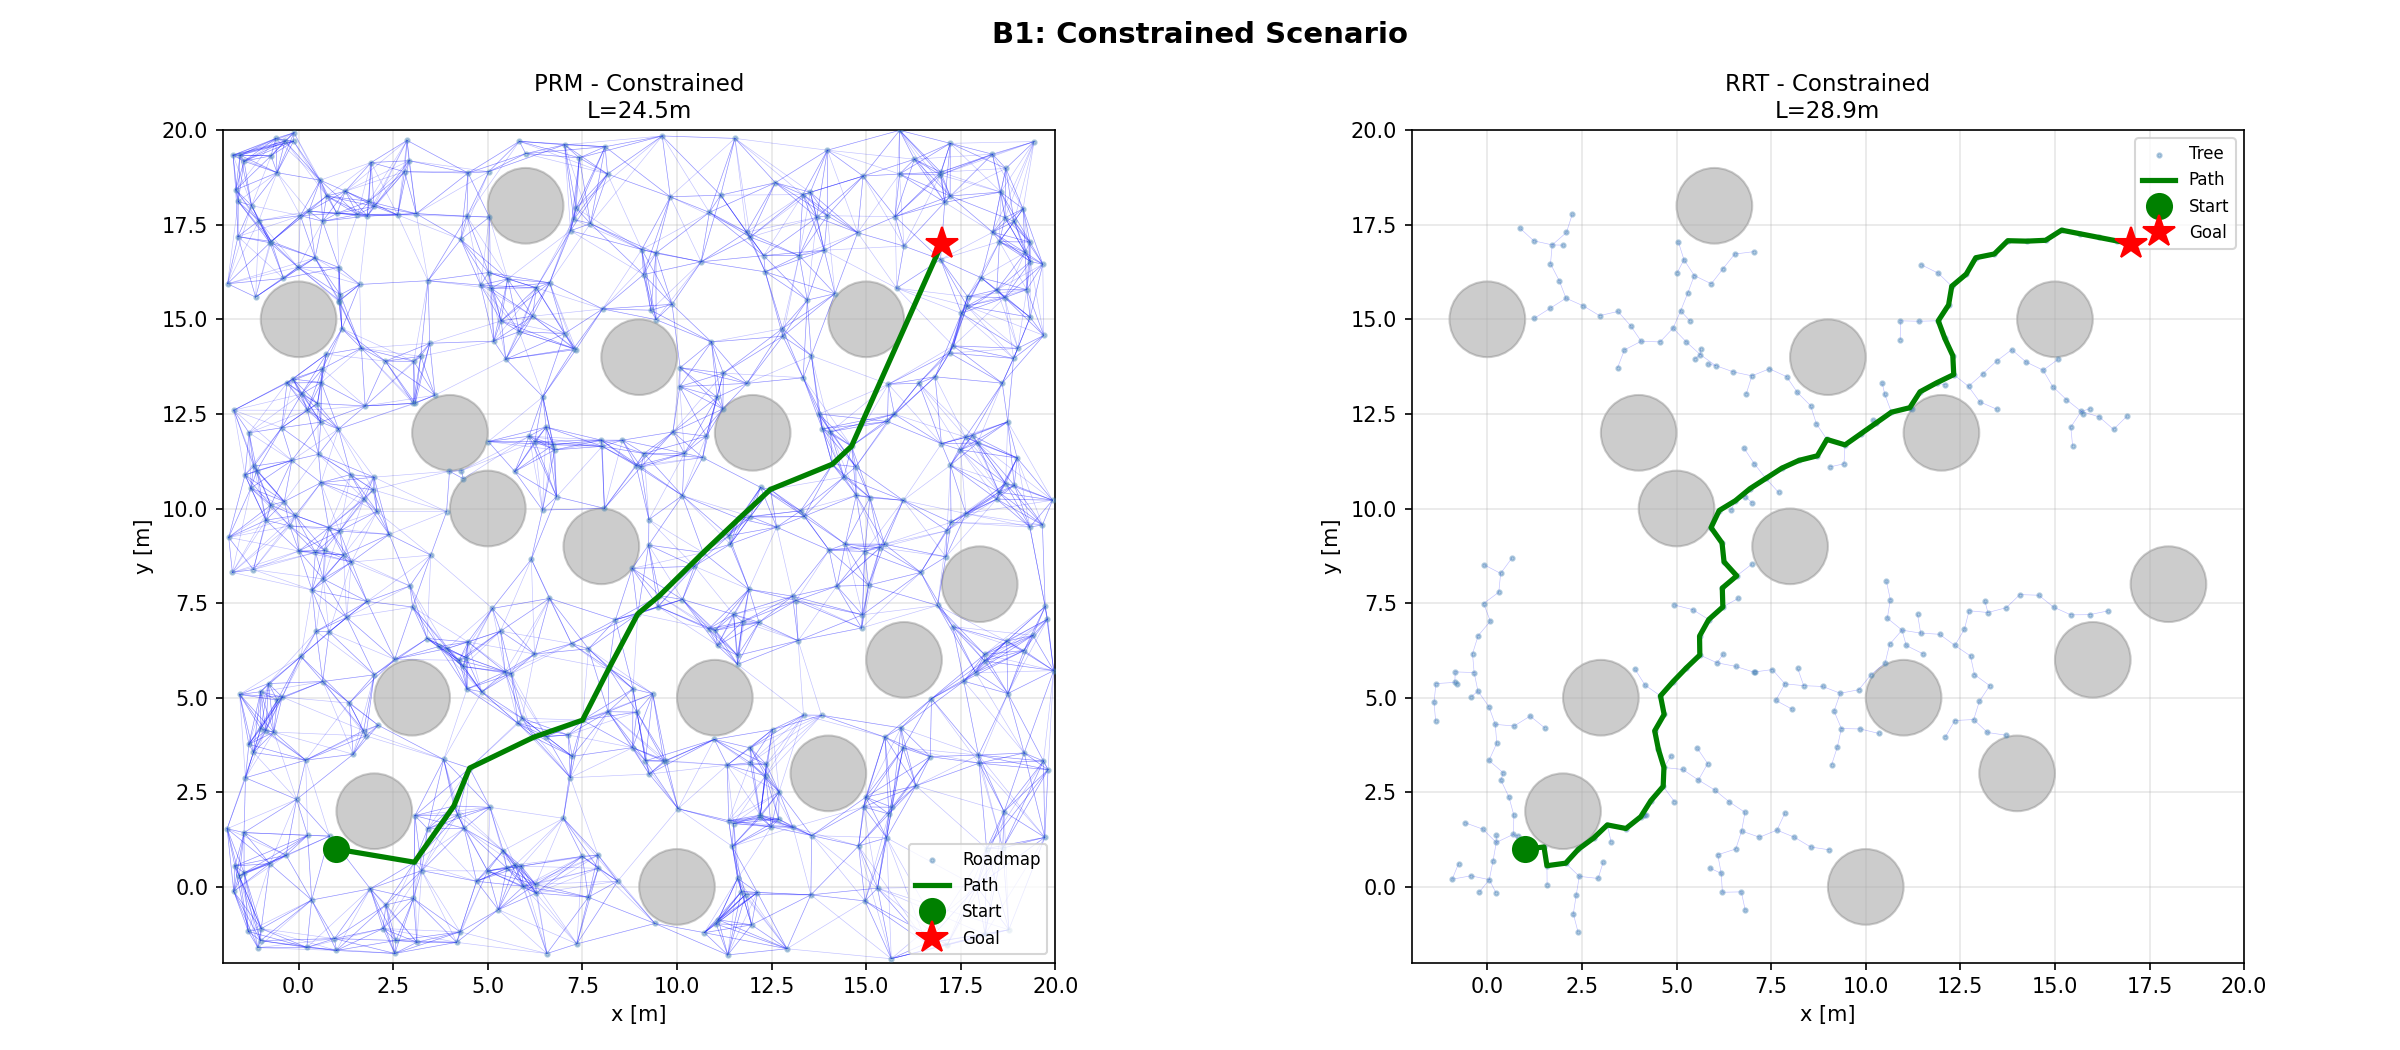
\includegraphics[width=0.6\textwidth]{results/partB/b1_constrained.png}
\caption{Constrained scenario. PRM (left) and RRT (right) with obstacle radius 1.0.}
\label{fig:b1}
\end{figure}

\subsection{B2.\ Metrics Comparison (Constrained, $N{=}30$)}

\begin{table}[ht]
\centering\small
\begin{tabular}{@{}lcc@{}}
\toprule
\textbf{Metric} & \textbf{PRM} & \textbf{RRT} \\
\midrule
Success rate & 100\% & 100\% \\
Avg path length & 24.48\,m & 28.72\,m \\
Avg time & 1.762\,s & 0.068\,s \\
Avg nodes & 500 & 217 \\
\bottomrule
\end{tabular}
\caption{B2 metrics (constrained scenario, 30 trials).}
\label{tab:b2}
\end{table}

Both achieve 100\% success. PRM produces 15\% shorter paths because A* finds the optimal route on the roadmap. RRT is $26\times$ faster because it does not build a full graph. The RRT paths zigzag visibly (\cref{fig:b1}, right) because each extension steps toward a random sample. PRM's A* finds the shortest graph path through dense collision-free nodes. This is the core trade-off: PRM gives better paths but costs more time. RRT is fast but paths need post-processing.

\subsection{B3.\ Parameter Studies}

\begin{table}[ht]
\centering\small
\begin{tabular}{@{}lcc@{\qquad\qquad}lcc@{}}
\toprule
\multicolumn{3}{c}{\textbf{PRM: n\_samples}} & \multicolumn{3}{c}{\textbf{RRT: goal\_sample\_rate}} \\
\cmidrule(r){1-3} \cmidrule(l){4-6}
\texttt{n\_samples} & Succ. & Avg Len & \texttt{goal\_rate} & Succ. & Avg Len \\
\midrule
100 & 100\% & 25.17\,m & 0.0 & 95\% & 29.97\,m \\
200 & 100\% & 24.85\,m & 0.1 & 100\% & 28.72\,m \\
400 & 100\% & 24.57\,m & 0.3 & 100\% & 28.10\,m \\
800 & 100\% & 24.27\,m & 0.7 & 100\% & 26.84\,m \\
\bottomrule
\end{tabular}
\caption{B3 parameter studies. PRM: $8\times$ more samples gives only 3.6\% shorter paths. RRT: goal bias is the strongest factor.}
\label{tab:b3}
\end{table}

\textbf{PRM:} Going from 100 to 800 samples only shortens paths by 3.6\%. The roadmap is dense enough at 200--400 nodes. More samples just add planning time.

\textbf{RRT step\_size:} Minimal effect (28.40--28.98\,m across 0.2--1.0). Smaller steps avoid obstacles better but need more iterations.

\textbf{RRT goal\_sample\_rate:} This is the most impactful parameter. Zero bias drops success to 95\% because the tree explores randomly. A 0.7 bias yields 10\% shorter paths by steering growth toward the goal. High bias works here because the direct route is mostly clear. In cluttered environments, high bias would waste iterations trying to extend through blocked areas.

% ===================================================================
\section{Part C: Improving PRM and RRT}
% ===================================================================

\textbf{Improvement: path shortcutting.}
I added a post-processing step to both planners. For 200 iterations, randomly pick two non-adjacent waypoints $i, j$. If the straight line between them is collision-free, remove all waypoints in between. This targets the main weakness of both planners: PRM paths follow graph edges that may detour, and RRT paths have many small incremental steps.

\noindent
\begin{minipage}[t]{0.42\textwidth}
\vspace{0pt}
\centering\small
\captionof{table}{Shortcutting results (20 trials).}
\label{tab:c}
\vspace{2pt}
\begin{tabular}{@{}lcccc@{}}
\toprule
 & \textbf{Before} & \textbf{After} & \textbf{Len $\Delta$} & \textbf{WP $\Delta$} \\
\midrule
PRM & 24.50\,m & 24.03\,m & $-2.0\%$ & $-69.5\%$ \\
RRT & 28.72\,m & 24.46\,m & $-14.8\%$ & $-90.9\%$ \\
\bottomrule
\end{tabular}
\end{minipage}%
\hfill
\begin{minipage}[t]{0.55\textwidth}
\vspace{0pt}
\centering
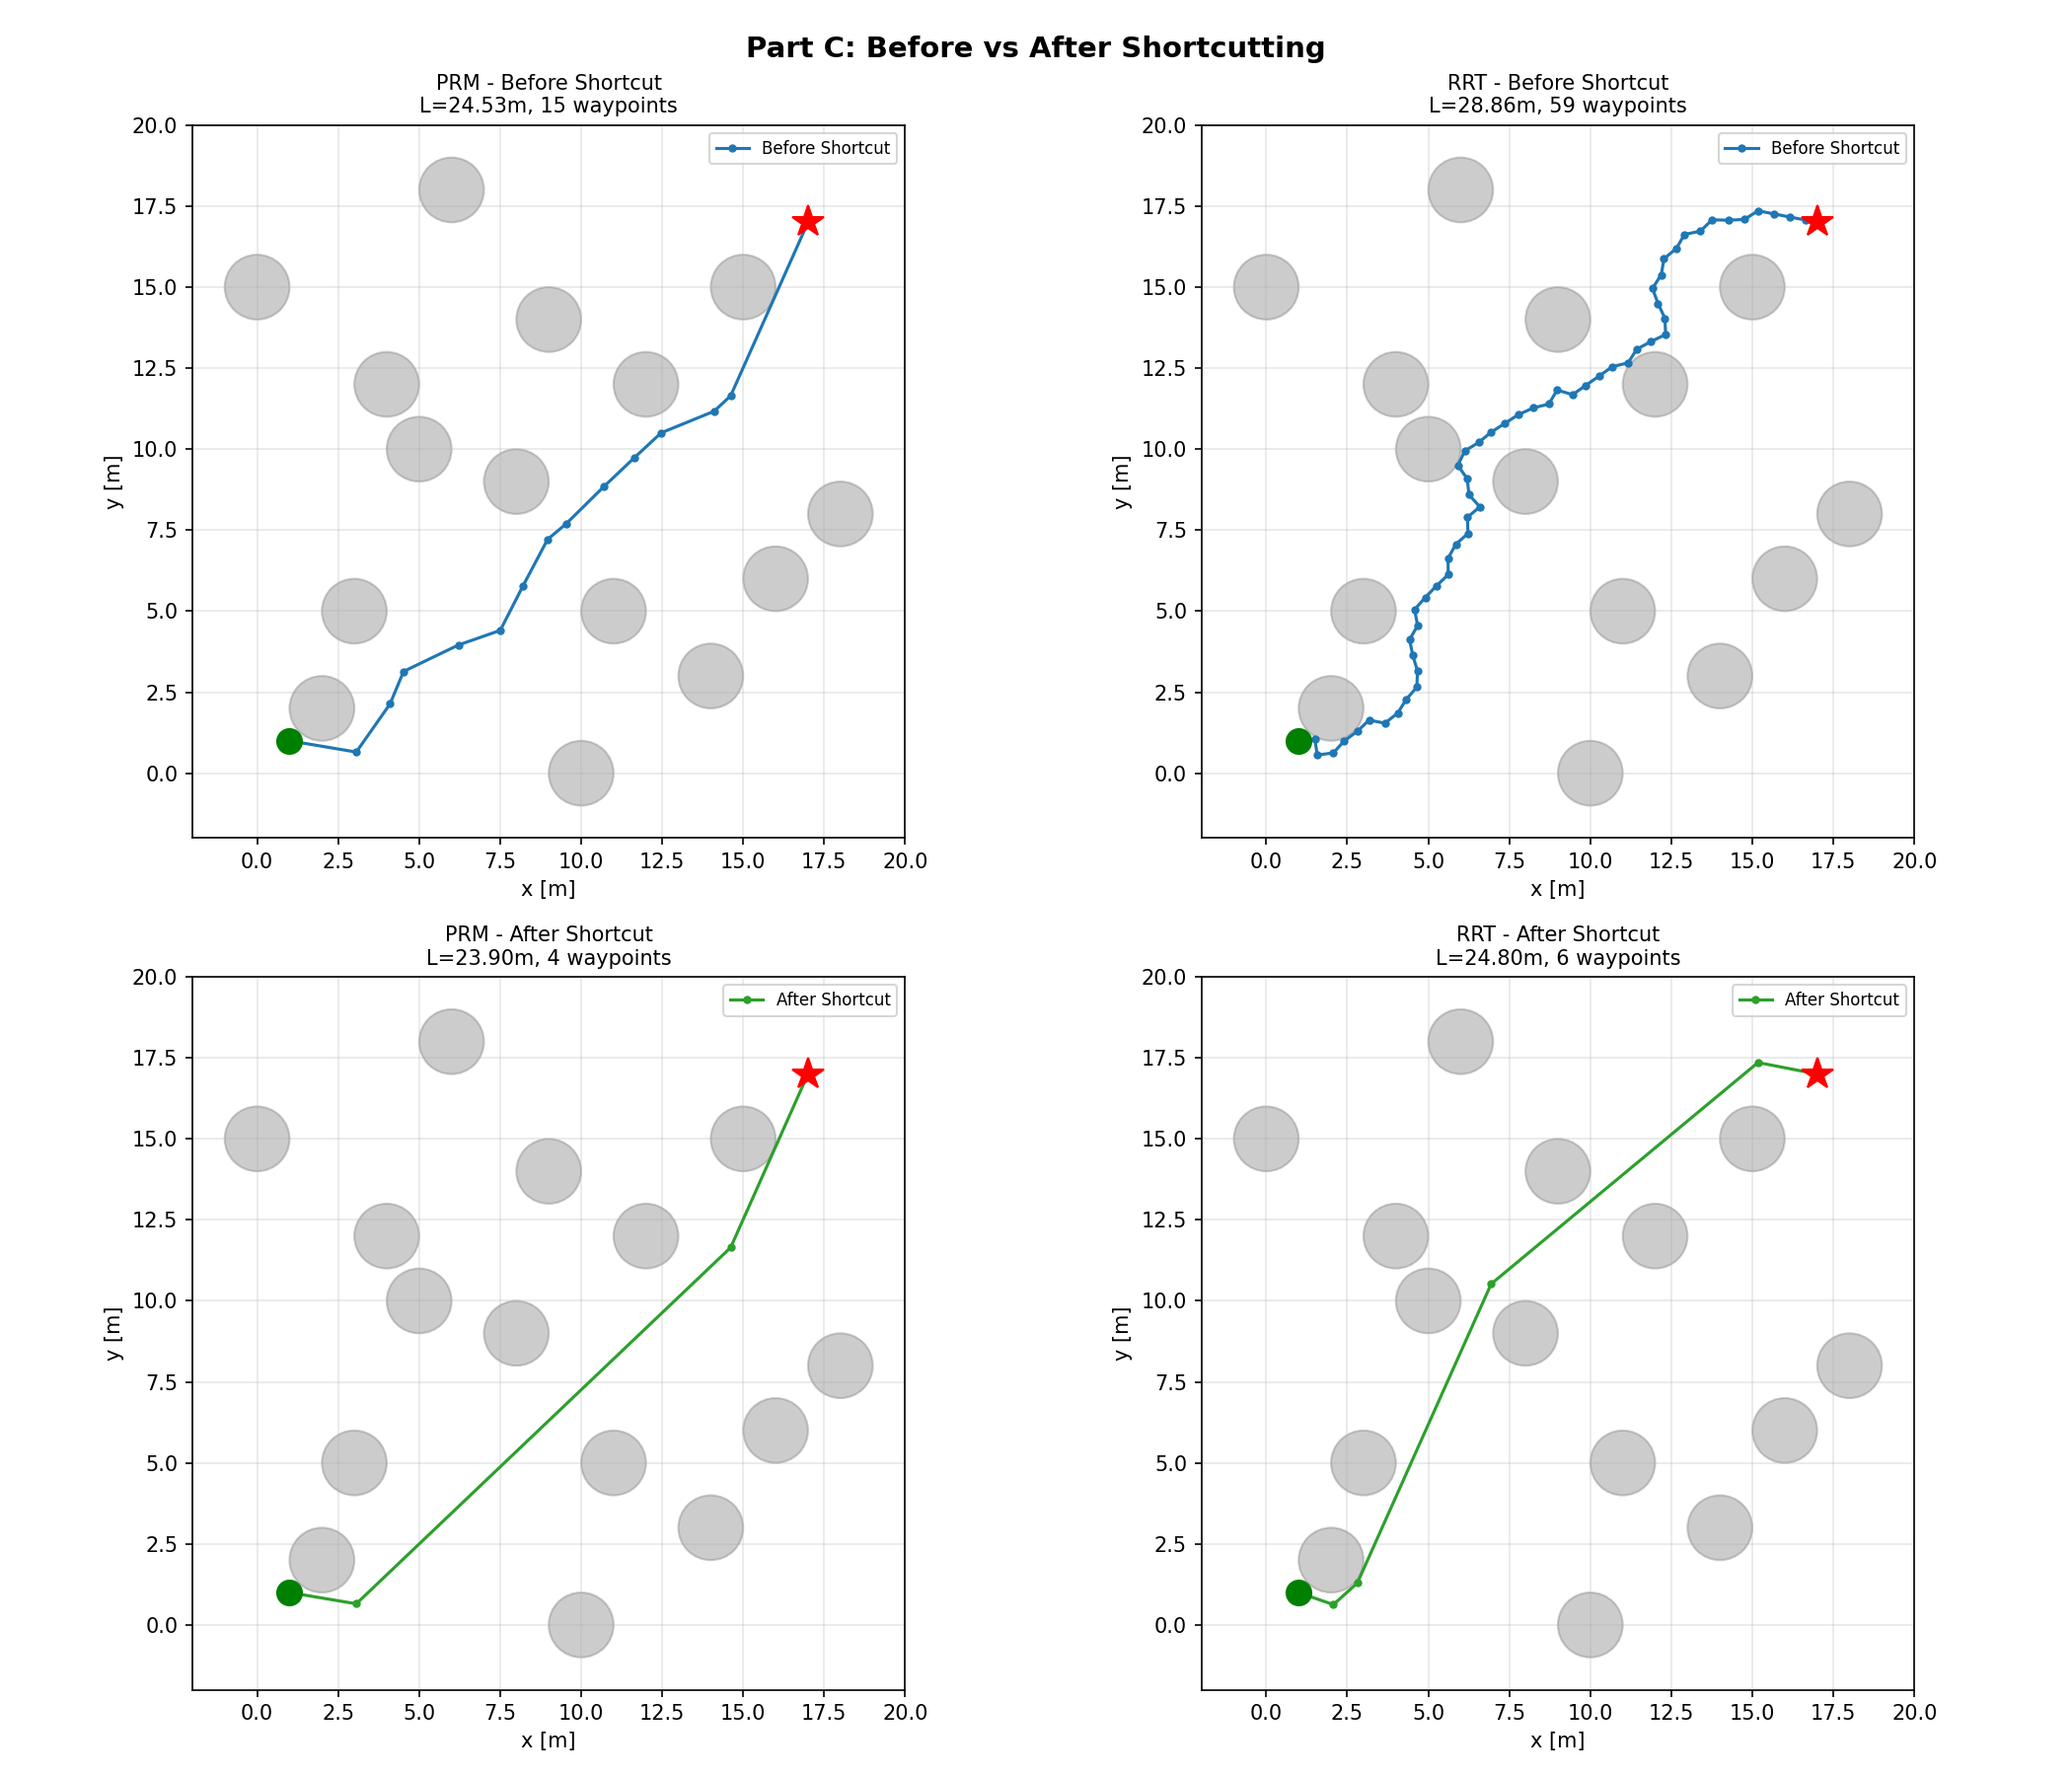
\includegraphics[width=\textwidth]{results/partC/c_before_after.png}
\captionof{figure}{Before (blue) vs.\ after (green) shortcutting. RRT (right) shows large simplification.}
\label{fig:c}
\end{minipage}

\vspace{4pt}
RRT benefits the most: 14.8\% shorter paths and 91\% fewer waypoints, because its small incremental steps are easy to shortcut into long straight segments. PRM improves less in length ($-2.0\%$) since A* already gives near-optimal paths, but still drops 70\% of waypoints. After shortcutting, both planners produce paths around 24\,m, which is likely close to the true shortest collision-free path. This means the planner choice matters less once post-processing is applied. In practice, RRT ($26\times$ faster) combined with shortcutting can match PRM's path quality at much lower cost.

\subsection*{Use of AI Tools}
{\small I used Claude Code to write experiment scripts and plotting code. I designed the experiments, verified outputs, and wrote all analysis myself.}

\end{document}
